\section{Results and Discussion}\label{sec:results}

\subsection{Dataset description}\label{sec:data}

The benchmark contains 1,000 constructed claim--photograph pairs, each combining one CarDD photograph~\cite{wang2023cardd} (4,000 photographs, over 9,000 annotated damage instances in six categories; research use with consent, no redistribution) with one record from the public Auto Insurance Claims data set~\cite{kaggleclaims} (licence not verified; used for research only and not redistributed). Each source item is used once, after duplicate photographs were removed. Each pair has one JPEG, the \texttt{claim\_description} text and eleven numerical fields (total, vehicle, injury and property amounts, deductible, premium, age, months as a customer, model year, bodily injuries, witnesses), with no missing values. The vehicle in the text is not the one in the photograph, and the label records how a pair was built, not a real claim outcome. A stratified 70/15/15 split gives 700 training claims (189 approvals, 291 audits, 220 escalations) and 150 each for validation and test (41, 62, 47): 27.1\%, 41.5\% and 31.4\% overall. Twenty-eight test descriptions also occur in training.

\paragraph{How the labels were built.}
The labels follow documented rules (Table~\ref{tab:rules}). Damage extent is the area of the union of CarDD boxes: surface damage covering at most 12\% of the image is \emph{localized}, damage covering at least 24\% with several boxes or a non-surface type is \emph{extensive}, the rest \emph{moderate}. Theft appears only among escalations, a total loss never among approvals, an unrecorded police report never among approvals, and every escalation photograph, and no other, was artificially degraded. The degradation also separates the two referral classes: 155 of the 343 claims with an unrecorded report are audits with clear photographs, and among 556 claims reporting major damage or a total loss, 390 audits and 103 escalations differ only in degradation. Table~\ref{tab:rules} counts escalations once in the order unrecorded report, theft, scope review (94 involve a theft and 103 a scope review). The build files were not kept, so the construction order cannot be confirmed. Approvals do not resemble straight-through claims (267 of 271 include an injury amount; median total US\$57,970), and an audit marks a severity mismatch, not fraud, so these are construction labels. The \texttt{pairing\_reason} field is never given to any model.

\begin{table}[!htb]
\caption{Label construction rules and their counts (all 1,000 claims).}\label{tab:rules}
\footnotesize
\begin{tabular*}{\textwidth}{@{\extracolsep{\fill}}>{\raggedright\arraybackslash}p{2.4cm}>{\raggedright\arraybackslash}p{6.9cm}r@{}}
\toprule
Label & Rule & Count \\
\midrule
Auto-Approve & Source claim not fraud-flagged, police status recorded; clear photograph whose extent is compatible with the reported severity (trivial with localized, minor with localized or moderate, major with extensive) & 271 \\
Reject/Fraud-Audit & Clear photograph whose extent differs from the reported severity: major damage or total loss with localized damage (390), or a fraud-flagged minor or trivial claim with extensive damage (25) & 415 \\
Escalate-Human & Missing or ambiguous evidence, counted once in order of precedence (police status unrecorded 188, otherwise theft 64, otherwise damage scope needing review 62), with the photograph degraded by blur, low light or a heavy crop & 314 \\
\botrule
\end{tabular*}
\end{table}

\subsection{Hardware and software specifications}\label{sec:setup}

Local computation ran on an Apple M1 (8 cores; GPU via MPS only for CLIP) with 8\,GB RAM under macOS 27.0.1, using Python 3.12.16 with NumPy 2.5.5, pandas 3.1.1, scikit-learn 1.9.1, SciPy 1.18.1, XGBoost 3.4.1, PyTorch 2.15.0, Transformers 5.24.0, Pillow 13.0.0 and matplotlib 3.11.2 (all versions in the repository lock file). Decision~1 (\texttt{gemini-decision-1}) was called through the Gemini Decisions REST API (\texttt{v1beta}) and Gemini 3.8 Flash through \texttt{generateContent}, from Amaravati, India, on 24 November 2026. Latencies are wall-clock times of sequential requests including the network round trip. Costs use the list prices on that date: US\$0.10 per million input tokens for Decision~1, with no output tokens, and US\$0.75 and US\$3.75 per million input and output tokens for Gemini 3.8 Flash, whose thinking tokens are billed as output.

\subsection{Comparison with baseline models}\label{sec:baselines}

All comparators share the proposed method's data, gate and threshold selection: B1--B3 measure each modality alone, B4 is the strongest conventional fusion model, B5 and B5-fair are generative, and the text rule and image-quality detector show how far the construction rules alone go.

\subsection{Evaluation metrics}\label{sec:metrics}

Let $n$ be the number of claims, $y_i$ the true route, $\hat{y}_i$ the predicted route before gating, $g_i$ the gated decision and $c_i$ the confidence. \textbf{Accuracy} is the share of correct predicted routes, and \textbf{Macro-F1} averages the per-class F1 so that small classes count equally:
\begin{equation}
\mathrm{Acc}=\frac{1}{n}\sum_{i=1}^{n}\mathbb{1}[\hat{y}_i=y_i],\qquad \text{Macro-F1}=\frac{1}{3}\sum_{k\in\mathcal{Y}}\frac{2P_kR_k}{P_k+R_k},
\end{equation}
where $P_k=\mathrm{TP}_k/(\mathrm{TP}_k+\mathrm{FP}_k)$ and $R_k=\mathrm{TP}_k/(\mathrm{TP}_k+\mathrm{FN}_k)$ are the precision and recall of class $k$ from its true positives, false positives and false negatives. \textbf{Expected calibration error} measures the gap between confidence and accuracy over $B=10$ equal-width confidence bins $B_b$~\cite{naeini2015,guo2017calibration}, and the \textbf{Brier score} is the mean squared error of the class probabilities~\cite{brier1950}:
\begin{equation}
\mathrm{ECE}=\sum_{b=1}^{B}\frac{|B_b|}{n}\,\big|\mathrm{acc}(B_b)-\mathrm{conf}(B_b)\big|,\qquad \mathrm{BS}=\frac{1}{n}\sum_{i=1}^{n}\sum_{y\in\mathcal{Y}}\big(h_y(\mathbf{z}_i)-\mathbb{1}[y_i=y]\big)^2,
\end{equation}
where $\mathrm{acc}(B_b)$ and $\mathrm{conf}(B_b)$ are the accuracy and mean confidence in bin $b$; ECE is compared with the 95th percentile of ECE for a perfectly calibrated model (labels drawn 1,000 times from the model's probabilities). \textbf{AURC}~\cite{geifman2017selective} averages, over $k$, the error rate among the $k$ most confident $\mathsf{A}$/$\mathsf{R}$ predictions. The \textbf{misrouting cost} is $\bar{C}=\frac{1}{n}\sum_i C(y_i,g_i)$ (Eq.~\ref{eq:cost}); \textbf{coverage} is $\frac{1}{n}\sum_i\mathbb{1}[g_i\neq\mathsf{E}]$, the \textbf{straight-through} share $\frac{1}{n}\sum_i\mathbb{1}[g_i=\mathsf{A}]$ counts the only claims no person handles, and \textbf{wrong approvals} are $\sum_i\mathbb{1}[g_i=\mathsf{A},y_i\neq\mathsf{A}]$. Two \textbf{handling-cost} variants charge for human work: in H1 each audit or escalation costs 1 and a wrong approval 10 (escalating everything costs 1); H2 charges 2 per audit and adds 4 for auditing a legitimate claim. \textbf{Efficiency} is the median latency and the cost per 1,000 claims, $1000\cdot\frac{1}{n}\sum_i\kappa_i$ (Eq.~\ref{eq:apicost}).

\textbf{Inference.} Test accuracy differences use the exact McNemar test with Holm correction over a family (proposed against B1, B3 and B4) chosen during revision, after the test results were known; test cost differences use paired bootstrap intervals (10,000 resamples); cross-validation differences use the corrected $t$-test; learning-curve differences a bootstrap over draws and claims (5,000 resamples).

\subsection{Implementation details and GitHub repository}\label{sec:impl}

A Decision~1 request averages 1,087 input tokens (536 for the image; JPEG quality 90). The combiner uses L-BFGS; validation selected $C=100$, at the grid edge (a grid to $10^5$ selects the same value), and the gate search at $(10,4,1)$ selected $\tau_c=0.85$, $\tau_s=0$. B1 and B3 use $C=10$; B2 and B4 use XGBoost (learning rate 0.05, subsampling 0.9; depth 3 with 200 trees and depth 6 with 200 trees) and B4 a 64-component SVD of TF-IDF, all selected on validation. B5 and B5-fair use temperature 0 and a JSON schema (B5-fair: thinking budget 0, medium resolution, combiner $C=1$); no output failed to parse. All seeds are 42. Before the freeze, validation was used for a pilot, for $C$ and for choosing the tri-modal configuration; B5-fair, the controls, cross-validation, learning curves, handling-cost variants and the re-test were added after the test run in response to review. Code, prompts, frozen configurations, cached responses and the lock file are at \url{https://github.com/rajeshkadiyalaaa/Claim_detection_Mulimodel}; CarDD photographs are not redistributed.

\subsection{Experimental results, figures and interpretation}\label{sec:exp}

\paragraph{Fixed-split comparison.}
Table~\ref{tab:main} reports the frozen test evaluation together with B5-fair.

\begin{table}[!htb]
\caption{Test-split results ($n=150$), with thresholds and hyperparameters selected on validation. Cost: mean misrouting cost at weights $(10,4,1)$ after gating (escalating every claim costs 0.687). Cov.: automated coverage. WA: wrong approvals. AURC over $\mathsf{A}$/$\mathsf{R}$ predictions. Accuracy 95\% intervals: proposed [0.79, 0.91], no-numbers [0.83, 0.93], B4 [0.87, 0.95]. B5-fair was added after the frozen evaluation.}\label{tab:main}
\footnotesize
\begin{tabular*}{\textwidth}{@{\extracolsep{\fill}}lcccccccc@{}}
\toprule
Method & Acc. & Macro-F1 & ECE & Brier & AURC & Cost & Cov. & WA \\
\midrule
Proposed (tri-modal) & 0.853 & 0.852 & 0.042 & 0.208 & 0.078 & 0.473 & 0.50 & 3 \\
\quad no numbers & 0.880 & 0.880 & 0.063 & 0.203 & 0.069 & 0.573 & 0.34 & 3 \\
B1 text only & 0.747 & 0.753 & 0.062 & 0.328 & 0.183 & 0.660 & 0.03 & 0 \\
B2 numbers only & 0.427 & 0.361 & 0.131 & 0.650 & 0.558 & 0.687 & 0.00 & 0 \\
B3 image only & 0.727 & 0.704 & 0.057 & 0.345 & 0.273 & 0.673 & 0.01 & 0 \\
B4 early fusion & 0.913 & 0.913 & 0.040 & 0.134 & 0.047 & 0.473 & 0.63 & 5 \\
B5 generative & 0.513 & 0.371 & 0.445 & -- & -- & 0.687 & 0.00 & 0 \\
B5-fair + combiner & 0.813 & 0.806 & 0.066 & 0.270 & 0.093 & 0.647 & 0.40 & 4 \\
\botrule
\end{tabular*}
\end{table}

The proposed router beats text alone and image alone (McNemar $p=0.011$ and $0.007$; Holm 0.023 and 0.020). B4 is 6.0 points more accurate, unresolved on this split ($p=0.064$; 5 against 14 discordant claims), at equal gated cost (0.473), higher coverage (63\% against 50\%) and more wrong approvals (5 against 3), and it has the lowest error among automatable claims (AURC 0.047 against 0.078 and 0.093 for B5-fair). B5 by default never predicts Auto-Approve and escalates everything; B5-fair reaches 0.813, not separable from the proposed method ($p=0.286$). Coverage counts audits, which go to investigators: the router settles 30 claims (20\%) straight through, audits 45 and escalates 75, so people handle 80\%; B4 settles 39 (26\%); each makes three wrongful audits, two on legitimate claims. ECE does not rank the learned routers, since all lie below the perfect-calibration reference (0.042 against 0.069 for the router, 0.040 against 0.057 for B4) except B2 (0.131 against 0.114) and B5 (0.445). On this split neither the router nor B4 is separable in cost from escalating everything ($-0.213$ $[-0.433,\,+0.047]$ and $-0.213$ $[-0.480,\,+0.113]$); B1 saves $0.027$ $[0.007,\,0.053]$ by automating 4 claims.

\begin{table}[!htb]
\caption{Repeated stratified cross-validation ($5\times5$ folds, all 1,000 claims) at weights $(10,4,1)$, with thresholds chosen from cross-fitted predictions inside each training fold. Means over the 25 folds, standard deviation in parentheses. ST, Audit, Esc.: shares approved automatically, audited and escalated. WA: wrong approvals per fold of 200 claims. Main rows use $C=10$.}\label{tab:cv}
\footnotesize
\begin{tabular*}{\textwidth}{@{\extracolsep{\fill}}lcccccc@{}}
\toprule
Method & Acc. & Cost & ST & Audit & Esc. & WA \\
\midrule
Proposed (tri-modal) & 0.866 (0.019) & 0.440 (0.098) & 0.17 & 0.33 & 0.51 & 3.0 \\
\quad with frozen $C=100$ & 0.870 (0.020) & 0.423 (0.085) & 0.16 & 0.31 & 0.53 & 2.6 \\
\quad no numbers & 0.880 (0.022) & 0.454 (0.092) & 0.16 & 0.29 & 0.54 & 3.2 \\
B1 text only & 0.780 (0.026) & 0.687 (0.041) & 0.02 & 0.02 & 0.96 & 0.5 \\
B3 image only & 0.738 (0.026) & 0.696 (0.033) & 0.01 & 0.04 & 0.96 & 0.6 \\
B4 early fusion & 0.908 (0.020) & 0.457 (0.093) & 0.21 & 0.36 & 0.43 & 4.9 \\
B5-fair + combiner & 0.814 (0.027) & 0.522 (0.117) & 0.15 & 0.30 & 0.55 & 3.2 \\
Escalate every claim & -- & 0.686 (0.002) & 0.00 & 0.00 & 1.00 & 0.0 \\
\botrule
\end{tabular*}
\end{table}

\paragraph{Cross-validation over all 1,000 claims.}
Table~\ref{tab:cv} repeats the comparison on every claim, with corrected intervals 1.3 to 1.5 times wider than a bootstrap over claims. The router lowers misrouting cost against escalating everything by $0.246$ $[0.134,\,0.357]$ ($p<0.001$), as do B4 ($0.229$ $[0.123,\,0.335]$) and B5-fair ($0.164$ $[0.031,\,0.297]$), but not B1 or B3. B4 is 4.2 points more accurate $[1.3,\,7.2]$ ($p=0.006$), and the cost difference ($-0.017$, $[-0.143,\,+0.110]$, $p=0.79$) is unresolved. Decision~1's answers are 5.2 points more accurate routing features than Gemini 3.8 Flash's answers to the same questions $[2.5,\,7.9]$ ($p=0.001$), with an unresolved cost difference ($+0.081$ $[-0.020,\,+0.183]$, $p=0.11$); this compares two hosted models, not mechanisms. Dropping the numbers changes accuracy by $+1.4$ points $[-0.3,\,3.1]$. Validation, test and cross-validation agree (0.867, 0.853, 0.866 for the router; 0.927, 0.913, 0.908 for B4).

\paragraph{Label efficiency.}
Figure~\ref{fig:lc} shows accuracy and gated cost as labels grow. The questions carry the construction rules, which are strong: the zero-label text rule reaches 0.723, above B4 with 25 or 50 labels and close to it with 100 (0.737). With 25 labels the router reaches 0.825, the rule-aware learner on text and image statistics 0.754, the text-only learner 0.728, B5-fair 0.786 and B4 0.609; the router leads the stronger rule-aware learner by 7.1 points $[1.4,\,12.9]$, B4 by 21.6 $[15.6,\,27.2]$ and B5-fair by 3.9 $[-0.2,\,8.0]$. The rule-aware learner overtakes the router at about 400 labels (0.869 against 0.864; 0.880 at 700, when B4 reaches 0.913), and on approvals and audits the text-only learner leads from 50 labels (0.855 against 0.822). At 25 labels the router's gated cost (0.704) is no better than escalating everything (0.687; B4 1.003); from 50 to 400 labels it is the lowest (0.590 at 50, 0.524 at 100), and B4 matches it only at 700 (0.487 against 0.503). Regularised B4 variants do no better at 25 claims (0.604--0.605). Most of the router's early lead over B4 is therefore rule knowledge in the questions.

\begin{figure}[!htb]
\centering
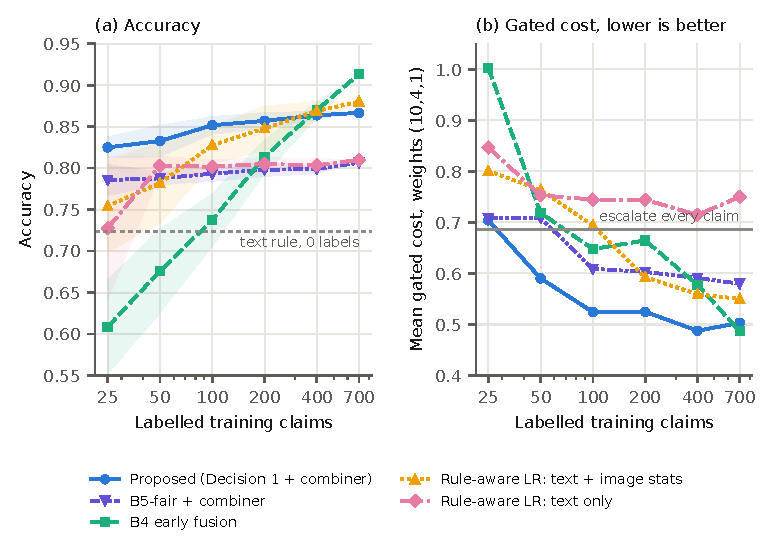
\includegraphics[width=\textwidth]{figures/fig_learning_curve.pdf}
\caption{Accuracy (a) and mean gated cost at weights $(10,4,1)$ (b) against the number of labelled training claims, on the 300 validation and test claims (ten stratified draws per size; shading in (a) is one standard deviation). Thresholds come from cross-fitted predictions inside each subsample. The rule-aware learners use features chosen with knowledge of the construction rules. B1 and B3 stay at or below 0.75 accuracy and are omitted.}\label{fig:lc}
\end{figure}

\paragraph{Efficiency.}
Decision~1 answers in a median of 0.80\,s (90th percentile 1.12\,s) with 1,087 input and no output tokens, about US\$0.11 per 1,000 claims; B5-fair takes 6.70\,s (10.10\,s) with 938 input and 335 output tokens, US\$1.96 (8.4 and 18 times more), and default B5 5.89\,s (8.18\,s) and US\$2.22. These are upper bounds, because the generative model still thought on 132 of 150 claims (243 tokens on average) despite a zero budget. Without thinking its median latency was 4.12\,s (about 5 times; 18 claims, not a random subset); default B5 is 7.4 times slower; answer tokens alone give 9.6 times the cost and input list prices alone 6.5 times. The advantage is thus about 5--8 times in speed and 6.5--18 times in cost, mostly list price, with runs eight hours apart; the absolute saving (about US\$1.85 per 1,000 claims and six seconds per claim) is small next to one human review.

\paragraph{Shortcut controls.}\label{sec:shortcuts}
Table~\ref{tab:short} applies the same checks to every method. The text rule equals the trained text model (0.747), and an image-quality detector separates escalations nearly as well as Decision~1's photograph check (AUC 0.932 against 0.957). On the matched subset, the text-based methods collapse, the image-only B3 scores highest (0.902 pooled, 0.909 on test), and the router and B4 tie at 0.805 (5 against 5 discordant claims); with 41 or 22 claims none of these differences is reliable. Degrading the clear photographs of the 103 test approvals and audits raised the share escalated from 28\% to 98\% (blur 100\%, low light 97\%, crop 97\%), and the photograph-clear answer fell from 0.51 to 0.19, near its 0.21 on true escalations. Without the 28 duplicated descriptions the router scores 0.844 and B4 0.926. Every method exploits construction rules, and the router's escalation route is largely a detector of the planted degradation.

\begin{table}[!htb]
\caption{Shortcut controls. Text rule: escalate theft or an unrecorded police report, audit a total loss, approve otherwise. A/R: the 103 test approvals and audits. Matched subset: approvals and audits reporting major damage with a recorded police status, pooled over validation and test (41 claims) and on test only (22).}\label{tab:short}
\footnotesize
\begin{tabular*}{\textwidth}{@{\extracolsep{\fill}}lcccc@{}}
\toprule
Method & Test acc. & A/R claims & Matched, val + test & Matched, test \\
\midrule
Text rule (no learning) & 0.747 & -- & 0.439 & -- \\
Proposed (tri-modal) & 0.853 & 0.825 & 0.805 & 0.682 \\
\quad no numbers & 0.880 & 0.845 & 0.902 & 0.818 \\
B1 text only & 0.747 & 0.757 & 0.341 & 0.318 \\
B3 image only & 0.727 & 0.631 & 0.902 & 0.909 \\
B4 early fusion & 0.913 & 0.883 & 0.805 & 0.773 \\
B5-fair + combiner & 0.813 & 0.777 & 0.585 & 0.545 \\
\botrule
\end{tabular*}
\end{table}

\paragraph{Ablations.}
In Table~\ref{tab:abl}, the routing question alone answers ``Fraud-Audit'' for almost every claim (0.427), so the combiner is essential and the checks carry most of the signal (0.867 alone). Removing the image costs 22 points and the text 15; the numbers add nothing (0.880 without them, $p=0.39$), as the labels never depend on amounts. Validation selected $\tau_s=0$, so the support term is unused. Cost differences between ablations are unreliable at 150 claims.

\begin{table}[!htb]
\caption{Ablations on the test split. Question ablations reuse the API responses and refit the combiner; modality ablations re-query Decision~1 without one input. Differences of a few points are within the noise of 150 claims.}\label{tab:abl}
\footnotesize
\begin{tabular*}{\textwidth}{@{\extracolsep{\fill}}lcccc@{}}
\toprule
Variant & Acc. & Macro-F1 & ECE & Cost \\
\midrule
Full method (tri-modal) & 0.853 & 0.852 & 0.042 & 0.473 \\
Routing question only, no combiner & 0.427 & 0.224 & 0.388 & 0.620 \\
Combiner on the routing question only & 0.647 & 0.571 & 0.091 & 0.620 \\
Combiner on the check questions only & 0.867 & 0.865 & 0.042 & 0.553 \\
Without $q_2$ / $q_3$ & 0.787 / 0.740 & 0.779 / 0.727 & 0.053 / 0.086 & 0.713 / 0.400 \\
Without $q_4$ / $q_5$ & 0.853 / 0.867 & 0.850 / 0.865 & 0.042 / 0.029 & 0.433 / 0.507 \\
Without the image / text & 0.633 / 0.707 & 0.592 / 0.673 & 0.103 / 0.089 & 0.660 / 0.660 \\
Without the numbers & 0.880 & 0.880 & 0.063 & 0.573 \\
Confidence-only gate ($\tau_s=0$) & 0.853 & 0.852 & 0.042 & 0.473 \\
\botrule
\end{tabular*}
\end{table}

\paragraph{Sensitivity to the cost model.}
Table~\ref{tab:cost} re-selects thresholds for each cost model. At weights of 5 to 10 times a review, both learned routers cost clearly less than escalating everything. At $(20,4,1)$ and $(20,8,1)$ the router's cross-validated advantage ($-0.120$ and $-0.105$) is unresolved and the fixed-split thresholds did not transfer; at $(50,10,1)$ every method escalates. Under handling cost no method is distinguishable from escalating everything: in H1 the router costs 0.975 against 1.000 ($-0.025$ $[-0.103,\,+0.053]$), settling 13\% of claims, and B4 1.010; in H2 the thresholds escalate almost everything. The router's advantage therefore rests on misrouting cost, in which correct audits and escalations are free, and the weights are assumptions.

\begin{table}[!htb]
\caption{Mean cost under each cost model, thresholds re-selected. Test: frozen gate, automated coverage in parentheses. CV: $5\times5$ cross-validation, confidence-only gate, straight-through share in parentheses; $^{*}$ corrected $p<0.05$ against escalating every claim.}\label{tab:cost}
\footnotesize
\begin{tabular*}{\textwidth}{@{\extracolsep{\fill}}lcccccc@{}}
\toprule
 & \multicolumn{3}{c}{Test ($n=150$)} & \multicolumn{3}{c}{Cross-validation} \\
\cmidrule(lr){2-4}\cmidrule(lr){5-7}
Cost model & Esc. all & Proposed & B4 & Esc. all & Proposed & B4 \\
\midrule
(5, 2, 1) & 0.687 & 0.307 (0.56) & 0.307 (0.69) & 0.686 & 0.296$^{*}$ (0.20) & 0.264$^{*}$ (0.25) \\
(10, 4, 1) & 0.687 & 0.473 (0.50) & 0.473 (0.63) & 0.686 & 0.440$^{*}$ (0.17) & 0.457$^{*}$ (0.21) \\
(20, 4, 1) & 0.687 & 0.633 (0.27) & 0.687 (0.00) & 0.686 & 0.566 (0.14) & 0.665 (0.10) \\
(20, 8, 1) & 0.687 & 0.713 (0.27) & 0.687 (0.00) & 0.686 & 0.581 (0.13) & 0.703 (0.08) \\
(50, 10, 1) & 0.687 & 0.733 (0.02) & 0.687 (0.00) & 0.686 & 0.734 (0.01) & 0.686 (0.00) \\
H1 (handling) & 1.000 & 1.033 (0.41) & 1.000 (0.00) & 1.000 & 0.975 (0.13) & 1.010 (0.02) \\
H2 (handling) & 1.000 & 1.000 (0.00) & 1.000 (0.00) & 1.000 & 1.013 (0.01) & 1.000 (0.00) \\
\botrule
\end{tabular*}
\end{table}

\paragraph{Error analysis and stability.}\label{sec:errors}
The most frequent error of both routers is a true audit predicted as an approval (9 of 22 errors for the router, 7 of 13 for B4; Fig.~\ref{fig:cm}). Every method misses the five test audits that pair a fraud-flagged minor claim with extensive damage, since the fraud flag is not an input, and B4's advantage concentrates in the police-status and total-loss subgroups decided by text rules. Re-sending the first 100 test claims eight hours later changed 6 of 53 automated decisions, all to escalation; only 10 responses were numerically identical and single answers moved by up to 0.197, and the re-test cannot detect changes over longer periods.

\begin{figure}[!htb]
\centering
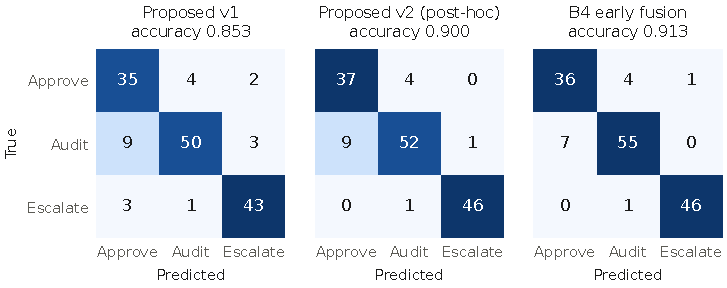
\includegraphics[width=0.85\textwidth]{figures/fig_confusion.pdf}
\caption{Test-set confusion matrices before gating, for the proposed method (v1), its post-hoc revision (v2) and early fusion (B4). Shading shows the row-normalised rate; numbers are counts.}\label{fig:cm}
\end{figure}

\paragraph{Post-hoc revision.}\label{sec:v2}
After the test evaluation, test errors showed that the routing question did not reflect the routing policy. A revised request (v2) states the routing rules, defines the options by visible evidence and adds police-status and theft questions. It raises zero-shot accuracy from 0.427 to 0.607 and, with the combiner, reaches 0.900 on test ($p=0.065$ against v1) and 0.897 in cross-validation (3.1 points above v1 $[0.5,\,5.7]$; $-1.1$ $[-3.4,\,+1.1]$ against B4). Test errors shaped it and its instruction restates the label rules, so v2 is exploratory.

\paragraph{Human oversight and limitations.}
People handle 80\% of claims at the default weights, and reviewer time and automation bias were not measured; the raw routing answer, almost always Fraud-Audit, should not be shown to reviewers, and an audit should be a triage flag, never an automated rejection. A degraded photograph alone triggers escalation, which would slow payment for claimants with poorer cameras, and identical requests can be routed differently, so each decision's scored response should be stored and audits should be contestable. Each decision sends the claimant's photograph and personal fields to an external service, which needs a lawful basis, retention terms and, for CarDD, the licensor's consent; every CarDD photograph in this study was sent to the Gemini API several times. Thresholds must be re-validated when the model changes, and automation should require a one-sided bound on the cost difference against escalate-all below zero. The study is limited by a small, constructed, rule-labelled benchmark with planted degradation, 150 test claims, a cost advantage that vanishes under handling cost, questions that carry the labelling rules, one proprietary model, efficiency ratios that are upper bounds, a 2026-only literature review, and analyses added after the test evaluation.
